\documentclass[a4paper,12pt]{extarticle}
\usepackage[utf8x]{inputenc}
\usepackage[T1,T2A]{fontenc}
\usepackage[russian]{babel}
\usepackage{hyperref}
\usepackage{indentfirst}
\usepackage{listings}
\usepackage{color}
\usepackage{here}
\usepackage{array}
\usepackage{multirow}
\usepackage{graphicx}
\usepackage{amsmath}
\usepackage{amssymb}

\usepackage{caption}
\renewcommand{\lstlistingname}{Программа} % заголовок листингов кода

\bibliographystyle{ugost2008ls}

\usepackage{listings}
\lstset{ %
extendedchars=\true,
keepspaces=true,
language=C,						% choose the language of the code
basicstyle=\footnotesize,		% the size of the fonts that are used for the code
numbers=left,					% where to put the line-numbers
numberstyle=\footnotesize,		% the size of the fonts that are used for the line-numbers
stepnumber=1,					% the step between two line-numbers. If it is 1 each line will be numbered
numbersep=5pt,					% how far the line-numbers are from the code
backgroundcolor=\color{white},	% choose the background color. You must add \usepackage{color}
showspaces=false				% show spaces adding particular underscores
showstringspaces=false,			% underline spaces within strings
showtabs=false,					% show tabs within strings adding particular underscores
frame=single,           		% adds a frame around the code
tabsize=2,						% sets default tabsize to 2 spaces
captionpos=t,					% sets the caption-position to top
breaklines=true,				% sets automatic line breaking
breakatwhitespace=false,		% sets if automatic breaks should only happen at whitespace
escapeinside={\%*}{*)},			% if you want to add a comment within your code
postbreak=\raisebox{0ex}[0ex][0ex]{\ensuremath{\color{red}\hookrightarrow\space}},
texcl=true,
inputpath=listings,                     % директория с листингами
}

\usepackage[left=2cm,right=2cm,
top=2cm,bottom=2cm,bindingoffset=0cm]{geometry}

%% Нумерация картинок по секциям
\usepackage{chngcntr}
\counterwithin{figure}{subsection}
\counterwithin{table}{section}

%%Точки нумерации заголовков
\usepackage{titlesec}
\titlelabel{\thetitle.\quad}
\usepackage[dotinlabels]{titletoc}

%% Оформления подписи рисунка
\addto\captionsrussian{\renewcommand{\figurename}{Рис.}}
\captionsetup[figure]{labelsep = period}

%% Подпись таблицы
\DeclareCaptionFormat{hfillstart}{\hfill#1#2#3\par}
\captionsetup[table]{format=hfillstart,labelsep=newline,justification=centering,skip=-10pt,textfont=bf}

%% Путь к каталогу с рисунками
\graphicspath{{fig/}}

\begin{document}	% начало документа

% Титульная страница
\begin{titlepage}	% начало титульной страницы

	\begin{center}		% выравнивание по центру

		\large Санкт-Петербургский Политехнический Университет Петра Великого\\
		\large Институт компьютерных наук и технологий \\
		\large Кафедра компьютерных систем и программных технологий\\[6cm]
		% название института, затем отступ 6см
		
		\huge Сети и телекоммуникации\\[0.5cm] % название работы, затем отступ 0,5см
		\large Отчет по лабораторной работе\\[0.1cm]
		\large  по сетевым технологиям\\[5cm]

	\end{center}


	\begin{flushright} % выравнивание по правому краю
		\begin{minipage}{0.25\textwidth} % врезка в половину ширины текста
			\begin{flushleft} % выровнять её содержимое по левому краю

				\large\textbf{Работу выполнил:}\\
				\large Болдырев А.В.\\
				\large {Группа:} 43501/3\\
				
				\large \textbf{Преподаватель:}\\
				\large Алексюк А.О.

			\end{flushleft}
		\end{minipage}
	\end{flushright}
	
	\vfill % заполнить всё доступное ниже пространство

	\begin{center}
	\large Санкт-Петербург\\
	\large \the\year % вывести дату
	\end{center} % закончить выравнивание по центру

\thispagestyle{empty} % не нумеровать страницу
\end{titlepage} % конец титульной страницы

\vfill % заполнить всё доступное ниже пространство

% Содержание
%% Содержание
\renewcommand\contentsname{\centerline{Содержание}}
\tableofcontents
\newpage


\section{Цель работы}
Ознакомиться с принципами программирования собственных протоколов, созданных на основе TCP и UDP.

\section{Краткое описание выполненных базовых работ по TCP и UDP}


В ходе выполнения лабораторных работ были написаны простейшие клиент-серверные приложения на базе протоколов TCP и UDP.
В приложениях TCP создается сокет, ставиться на прослушивание и при подключении клиента создается отдельный сокет, по которому клиент общается с сервером. 

Для инициализации, запуска и завершения TCP-сервера необходимо выполнить следующие системные вызовы:

\begin{enumerate}
\item socket() - создание сокета
\item bind() - привязка созданного сокета к заданным IP-адресам и портам
\item listen() – перевод сокета в состояние прослушивания
\item accept() - прием поступающих запросов на подключение и возврат сокета для нового соединения
\item recv() - чтение данных от клиента из сокета, полученного на предыдущем шаге
\item send() - отправка данных клиенту с помощью того же сокета
\item shutdown() - разрыв соединения с клиентом
\item close() - закрытие клиентского и слушающего сокетов
\end{enumerate}

TCP-клиенты выполняют следующую последовательность действий для открытия соединения, отправки и получения данных, и завершения:

\begin{enumerate}
\item socket() - создание сокета
\item connect() - установка соединения для сокета, который будет связан с серверным сокетом, порожденным вызовом accept()
\item send() - отправка данных серверу
\item recv() - прием данных от сервера
\item shutdown() - разрыв соединения с сервером
\item close() - закрытие сокета
\end{enumerate}

	Так же был реализован сервер, поддерживающий работу с несколькими клиентами.
Для этого при подключении клиента создается поток, который в котором создается сокет для общения с клиентом.
	
	В приложениях UDP сервер принимает сообщение от клиента и отправляет сообщение об успешной доставке. UDP протокол не подразумевает логических соединений, поэтому не создается слушающего сокета.

Реализация UDP-сервера имеет следующий вид:
\begin{enumerate}
\item socket() - создание сокета
\item bind() - привязка созданного сокета к заданным IP-адресам и портам
\item recvfrom() - получение данных от клиента, параметры которого заполняются функцией
\item sendto() - отправка данных с указанием параметров клиента, полученных на предыдущем шаге
\item close() - закрытие сокета
\end{enumerate}


UDP-клиент для обмена данными с UDP-сервером использует следующие функции:
\begin{enumerate}
\item socket() - создание сокета
\item recvfrom() - получение данных от сервера, параметры которого заполняются функцией
\item sendto() - отправка данных с указанием параметров сервера, полученных на предыдущем шаге
\item close() - закрывает сокет
\end{enumerate}


Проверено 2 способа написания клиента:
\begin{itemize}
\item С использованием функции connect
\item Без использования функции connect
\end{itemize}
В первом случае устанавливается соединение и клиент, и сервер работают аналогично TCP. Во втором случае при отсутствии доступа к серверу сообщение об ошибке не возникает, и клиент считает, что данные отправлены корректно.


\section{Индивидуальное задание}


Разработать приложение-клиент и приложение-сервер электронной почты. TCP-сервер реализован на Linux, TCP-клиент на Windows, UDP - наоборот. Реализация в зависимости от платформы будет различаться только в используемых библиотеках, так в Windows-реализации добавятся два системных вызова (WSAStartup(), WSACleanup()).

\textit{Основные возможности.}

Серверное приложение должно реализовывать следующие функции: 
\begin{enumerate}
\item Прослушивание определенного порта
\item Обработка запросов на подключение по этому порту от клиентов
\item Поддержка одновременной работы нескольких почтовых клиентов через механизм нитей
\item Приём почтового сообщения от одного клиента для другого
\item Хранение электронной почты для клиентов 
\item Посылка клиенту почтового сообщения по запросу с последующим удалением сообщения 
\item Посылка клиенту сведений о состоянии почтового ящика 
\item Обработка запрос на отключение клиента 
\item Принудительное отключение клиента
\end{enumerate}

Клиентское приложение должно реализовывать следующие функции:  
\begin{enumerate}
\item Установление соединения с сервером
\item Передача электронного письма на сервер для другого клиента
\item Проверка состояния своего почтового ящика
\item Получение конкретного письма с сервера
\item Разрыв соединения
\item Обработка ситуации отключения клиента сервером
\end{enumerate}

\textit{Настройки приложений.}
Разработанное клиентское приложение должно предоставлять пользователю настройку IP-адреса или доменного имени сервера электронной почты, номера порта, используемого сервером, идентификационной информации пользователя. Разработанное серверное приложение должно предоставлять пользователю настройку списка пользователей почтового сервера. 

\textit{Методика тестирования.}
Для тестирования приложений запускается сервер электронной почты и несколько клиентов. В процессе тестирования проверяются основные возможности приложений по передаче и приёму сообщений.

\section{Дополнительное задание}

Попробовать проанализировать код с помощью статического и динамического анализатора. Когда закончите индивидуальные задания, проверьте исходный код своих программ с помощью clang-tidy и cppcheck. При запуске утилит включайте все доступные проверки. После этого проверьте с помощью valgrind свои программы на предмет утечек памяти и неправильного использования многопоточности. Опишите все найденные ошибке в отчете, а также укажите, как их можно исправить. (в качестве средства анализа выбран PVS-studio)






\section{Разработанный прикладной протокол}

Основа протокола – файл API.h, хранящий закодированные команды enum-типа, а также строковые расшифровки этих команд.
Команды: 

START -> после посылки данной команды сервер отправляет код SERV\_OK, подтверждающий успешное создание соединения с клиентом.
INIT -> данное состояние существует только для отображения меню клиента (не аутентифицированного).
EXIT -> после посылки данной команды сервер отправляет код SERV\_OK, подтверждающий успешный разрыв соединения с клиентом и закрытие сокета.
REG [uname, passw] -> после посылки данной команды и указанных аргументов сервер отправляет код SERV\_OK, подтверждающий успешное создание учетной записи пользователя.
LOG [uname, passw] -> после посылки данной команды и указанных аргументов сервер отправляет код SERV\_OK, подтверждающий успешный вход в заданную учетную запись.
LUG -> после посылки данной команды сервер отправляет код SERV\_OK, подтверждающий успешный выход клиента из учетной записи.
SND [uname, mes] -> после посылки данной команды и указанных аргументов сервер отправляет код SERV\_OK, подтверждающий успешное создание сообщения и отправки его указанному клиенту.
DEL\_US -> после посылки данной команды сервер отправляет код SERV\_OK, подтверждающий успешное удаление пользователя (удаление только учетной записи пользователя, находящегося в системе).
DEL\_MES [mesID] -> после посылки данной команды сервер отправляет код SERV\_OK, подтверждающий успешное удаление сообщения с данным ID.
SH\_UNR -> после посылки данной команды сервер отправляет код SERV\_OK, а также все непрочитанные сообщения из почтового ящика.
SH\_ALL -> после посылки данной команды сервер отправляет код SERV\_OK, а также все сообщения из почтового ящика.
SH\_EX [mesID] -> после посылки данной команды сервер отправляет код SERV\_OK, а также конкретное сообщение из почтового ящика по данному ID.
RSND [uname, mesID] -> после посылки данной команды сервер отправляет код SERV\_OK, подтверждающий успешную пересылку сообщения одним пользователем другому. 
INSYS -> данное состояние существует только для отображения меню клиента (аутентифицированного).

Также во всех указанных случаях сервер имеет возможность послать ответ NO\_OPERATION, свидетельствующий об ошибке (например, либо выполнения операции на стороне сервера, либо о том, что были введены некорректные данные, и т.д.).

Все команды отправляются в формате <API[STATE]|numArg|\{args|\}|>
Все сообщения отправляются в формате $\hat{}$<id>$\hat{}$<from>$\hat{}$<date/time>$\hat{}$<len>$\hat{}$<state>$\hat{}$ , и могут в произвольном количестве передаваться в качестве аргументов. Как сообщения, так и команды сериализуются перед отправкой в строки и десериализуются после получения.

\begin{figure}[H]
	\begin{center}
		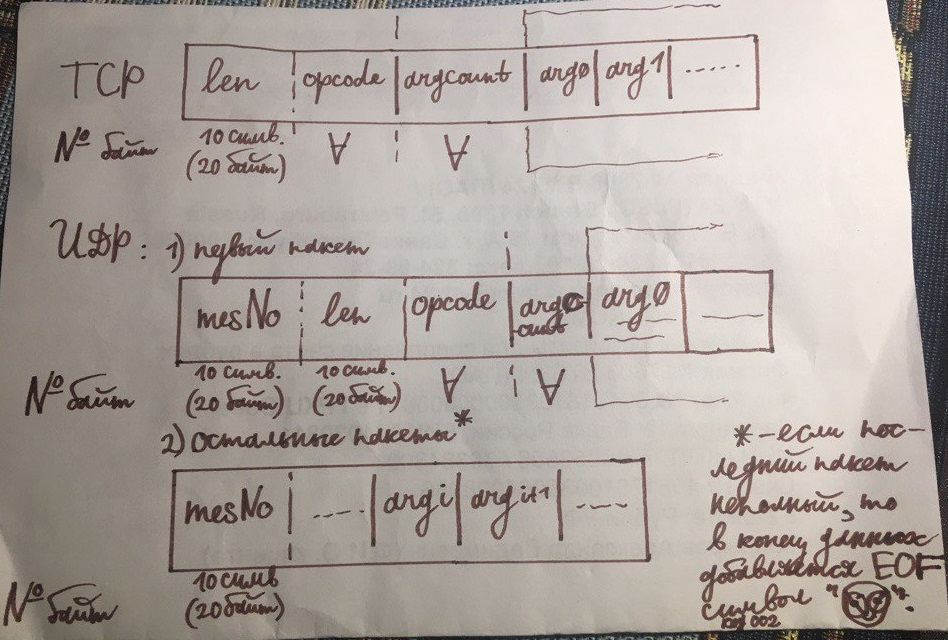
\includegraphics[scale=0.7]{format}
		\caption{Форматы пересылаемых пакетов для TCP и UDP реализаций} 
		\label{pic:format} % название для ссылок внутри кода
	\end{center}
\end{figure}
На данном рисунке представлен формат пакетов, передаваемых для TCP и UDP протоколов.
Стандартно, для TCP-варианта пакет содержит поле длины сообщения неизменной длины (10 символов, в 2-байтовой кодировке - 20 байт, здесь и далее), далее поле кода операции, количества аргументов и сами аргументы (их размер не фиксирован), а также разделители между нефиксированными полями.

Для UDP-варианта пакет содержит поле номера пакета (фиксированное), поле длины сообщения неизменной длины (фиксированное), далее поле кода операции, количества аргументов и сами аргументы (их размер не фиксирован), а также разделители между нефиксированными полями. В отличие от TCP, здесь пакеты делятся на передаваемые подпакеты равной длины, фиксируемой в протоколе (например, 1024 байта) - исходные пакеты делятся на подпакеты в соответствии с этим значением с учетом служебных полей номера пакета и длины. Поле длины присутствует только в первом передаваемом подпакете, в остальных - отсутствует. Если в самом последнем подпакете сообщения остается свободное пространство, во избежание приема мусора в конце данных этого подпакета вставляется спецсимвол окончания данных (код 002 ASCII).


\section{Тестирование приложения на основе TCP}

Для тестирования приложения запускался сервер и несколько клиентов. Проверялись все команды поддерживаемые сервером в различных комбинациях.
	В результате тестирования ошибок выявлено не было, из чего можно сделать вывод, что приложение работает корректно.


\section{Тестирование приложения на основе UDP}

Для тестирования приложения запускался сервер и несколько клиентов. Проверялись все команды поддерживаемые сервером в различных комбинациях.
	В результате тестирования ошибок выявлено не было, из чего можно сделать вывод, что приложение работает корректно.

\begin{figure}[H]
	\begin{center}
		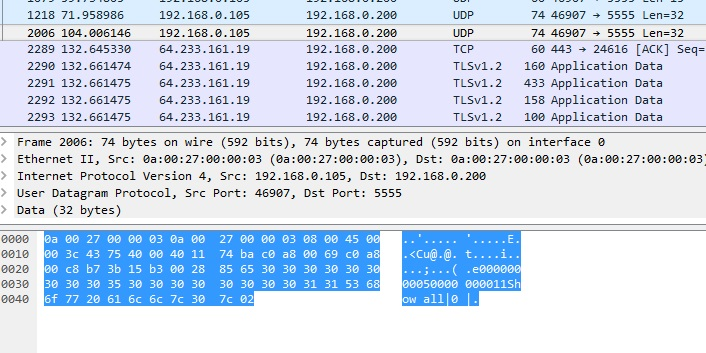
\includegraphics[scale=0.7]{wire}
		\caption{Пример наблюдения передаваемых пакетов в WireShark} 
		\label{pic:wire} % название для ссылок внутри кода
	\end{center}
\end{figure}

Как можно видеть на данном рисунке, по сети передаются пакеты по протоколу UDP, содержащие помимо служебной информации непосредственно передаваемые данные.

\begin{figure}[H]
	\begin{center}
		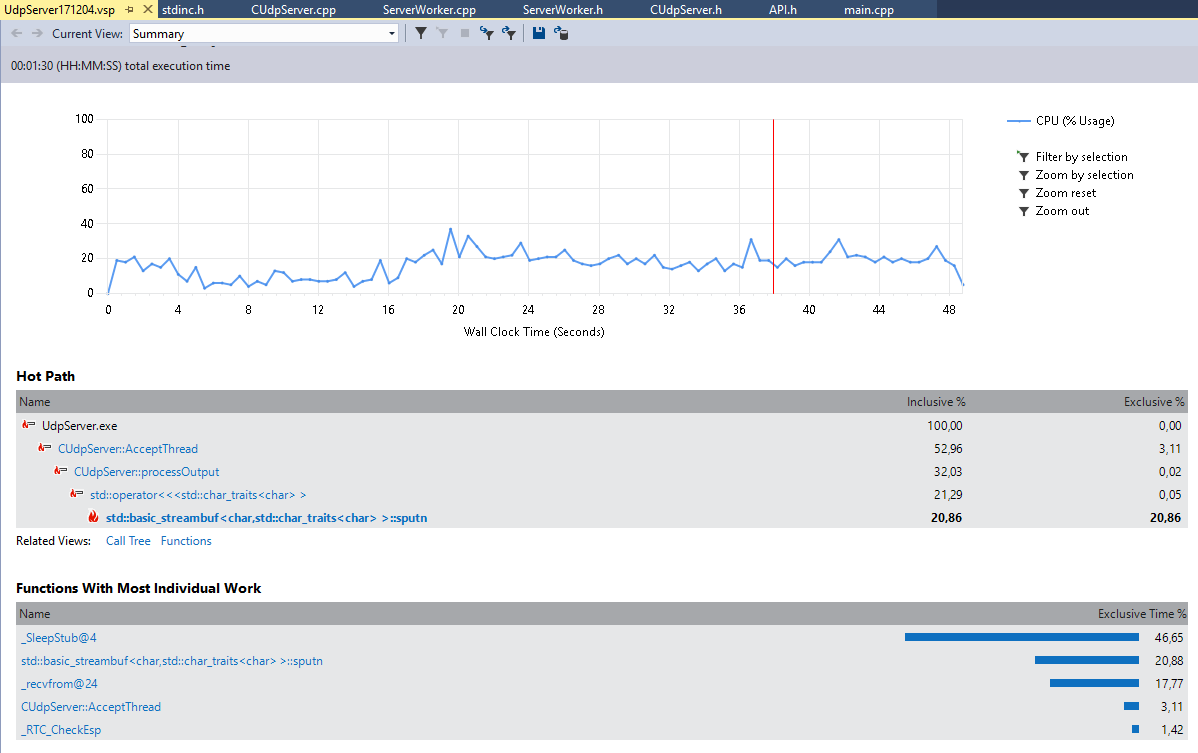
\includegraphics[scale=0.5]{profiler}
		\caption{Исследование узких мест приложения с помощью профайлера} 
		\label{pic:profiler} % название для ссылок внутри кода
	\end{center}
\end{figure}

С помощью профилировщика, встроенного в Visual Studio, было выявлено, что процессор в наибольшей степени обрабатывает запросы Sleep() и вывода информации на экран, после них - блокирующая функция recvfrom(). 

\section{Дополнительное задание}

В качестве средства статического и динамического анализа был выбран плагин PVS-studio для Visual Studio, пример для приложения UDPServer.

\begin{figure}[H]
	\begin{center}
		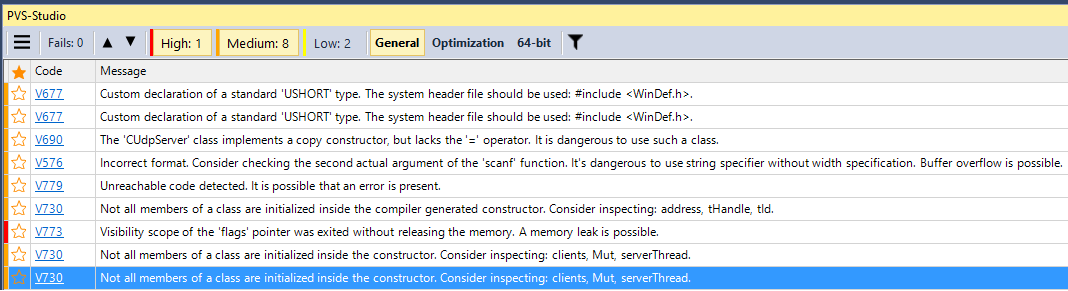
\includegraphics[scale=0.7]{pvs}
		\caption{Пример выводимых возможных уязвимостей приложения в PVS-Studio} 
		\label{pic:pvs} % название для ссылок внутри кода
	\end{center}
\end{figure}

В приложении замечена одна критическая и семь некритических уязвимостей. Критическая - утечка памяти, в связи с тем, что память, выделенная для flags, не освобождается. Решение - освобождать память путем вызова delete[] flags.
Остальные - например, переопределение типа USHORT, зарезервированного в системе - исправляется изменением имени типа. Другой пример - не все члены класса генерируются в конструкторе, сгенерированном компилятором. Решение - добавление явной инициализации соответствующих переменных в конструктор.

\section{Выводы}
В данной лабораторной работе было реализовано клиент-серверное приложение электронной почты. Данная система обеспечивает параллельную работу нескольких клиентов.

На примере данной разработки были изучены основные приемы использования протокола транспортного уровня TCP – транспортного механизма, предоставляющего поток данных, с предварительной установкой соединения, за счёт этого дающего уверенность в достоверности получаемых данных, осуществляющего повторный запрос данных в случае потери данных и устраняющего дублирование при получении двух копий одного пакета. Данный механизм, в отличие от UDP, гарантирует, что приложение получит данные точно в такой же последовательности, в какой они были отправлены, и без потерь. При подключении нового клиента создается новый сокет, что значительно упрощает создание многоклиентского приложения на основе нитей.

\section{Листинги программ}

Листинги программ находятся по адресу: 

https://github.com/AleksanderBoldyrev/TCP\_UDP\_MAIL.git

\end{document}

